%=========================================================================
% fig-background-cnn.tex
%=========================================================================

\begin{figure}[h]

  \centering
  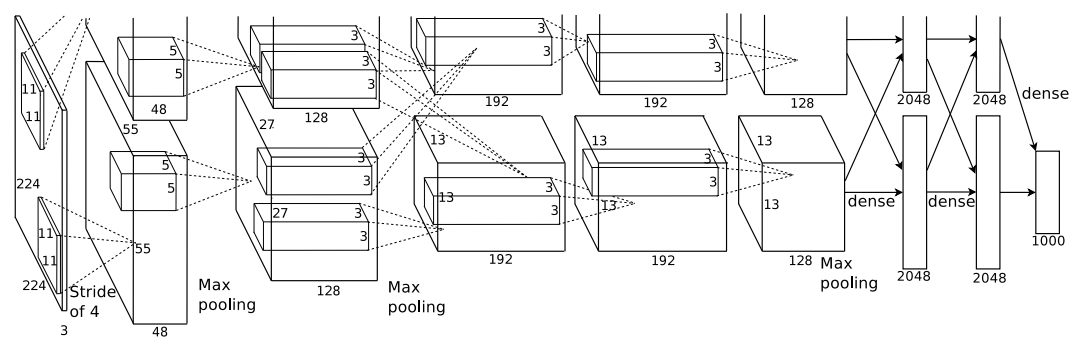
\includegraphics[width=0.9\tw]{fig-background-cnn.png}

  \caption{\textbf{Example CNN Pipeline --} The composition of layers in
    a CNN used for classifying images. A 224x244x3 (RGB-channels) input
    image is processed by five convolutional layers, two pooling layers,
    and two fully-connected layers to generate probabilities for 1000
    possible output labels. A. Krizhevsky, I. Sutskever,
    G. E. Hinton. ImageNet Classification with Deep Convolutional Neural
    Networks. NIPS 2012.}

  \label{fig-background-cnn}

\end{figure}
